\chapter{Meilensteinplanung}
Im Rahmen dieses Projekts wurde eine umfassende Planung und Organisation der Arbeitspakete durchgeführt. 
Dies umfasste die Analyse der Tabelle mit den Arbeitspaketen sowie die Erstellung eines Gantt-Diagramms. 
Letzteres bietet eine visuelle Darstellung der zeitlichen Abfolge und Dauer der verschiedenen Aufgaben, was die Projektplanung und -kontrolle erleichtert.

\section{Vorgehensweise zur Erstellung des Gantt-Diagramms}
Zunächst wurden allel relvanten Daten aus den Arbeitspaketen extrahiert und aufbereitet.
Die Tabelle enthielt zwei wesentliche Spalten, und zwar \enquote{Beschreibung} und \enquote{Dauer}.
Zur Erstellung des Gantt-Diagramms wurde die Website \texttt{onlinegantt.com} in Anspruch genommen.
Diese Plattform bietet eine benutzerfreundliche Oberfläche zur Eingabe und Visualisierung von Projektplänen. \newline
Für jedes Arbeitspaket wurde das Startdatum gemäß der Tabelle eingetragen.
Dabei wurde die Aufgabenbeschreibung wurde als Titel für die jeweiligen Arbeitspakete verwendet.
Die Dauer der Aufgaben wurde entsprechend der Tabelle kategorisiert, entweder in Tagen oder Wochen angegeben. \newline
Dadurch konnte die zeitliche Abfolge der Aufgaben visualisiert werden, um mögliche Überschneidungen oder Abhängigkeiten zwischen diesen zu erkennen. 
Die Erstellung des Gantt-Diagramms zeigte eine klare Struktur des Projekts mit einem Zeitrahmen vom 08.03.2024 bis 18.06.2024. 
Die logische und sequenzielle Anordnung der Aufgaben erleichtert die Nachverfolgung und Kontrolle des Projekts.

\section{Planung der Arbeitspakete}
Einige Aufgaben, wie in etwa der Einrichtung des GitHub-Repositories oder die Erstellung der Projektstruktur, beanspruchten lediglich einen Tag. 
Andere Aufgaben, wie die Implementierung des Chat-Screens oder die Anpassung der Seiten-Navigation, erstreckten sich über mehrere Wochen.
Diese umfangreicheren Aufgaben wurden in verschiedenen Sprints parallel zu den kürzeren Aufgaben geplant, um die Effizienz der Gesamtdauer des Projekts zu maximieren.

\section{Visualisierung}
Durch das Gantt-Diagramm konnten potenzielle Engpässe und Risiken identifiziert werden.
Ein besonderes Augenmerk galt Aufgaben, die kritische Pfade darstellen, um Verzögerungen zu vermeiden.

\begin{figure}[H]
    \caption[Meilensteinplanung]{Meilensteinplanung}
    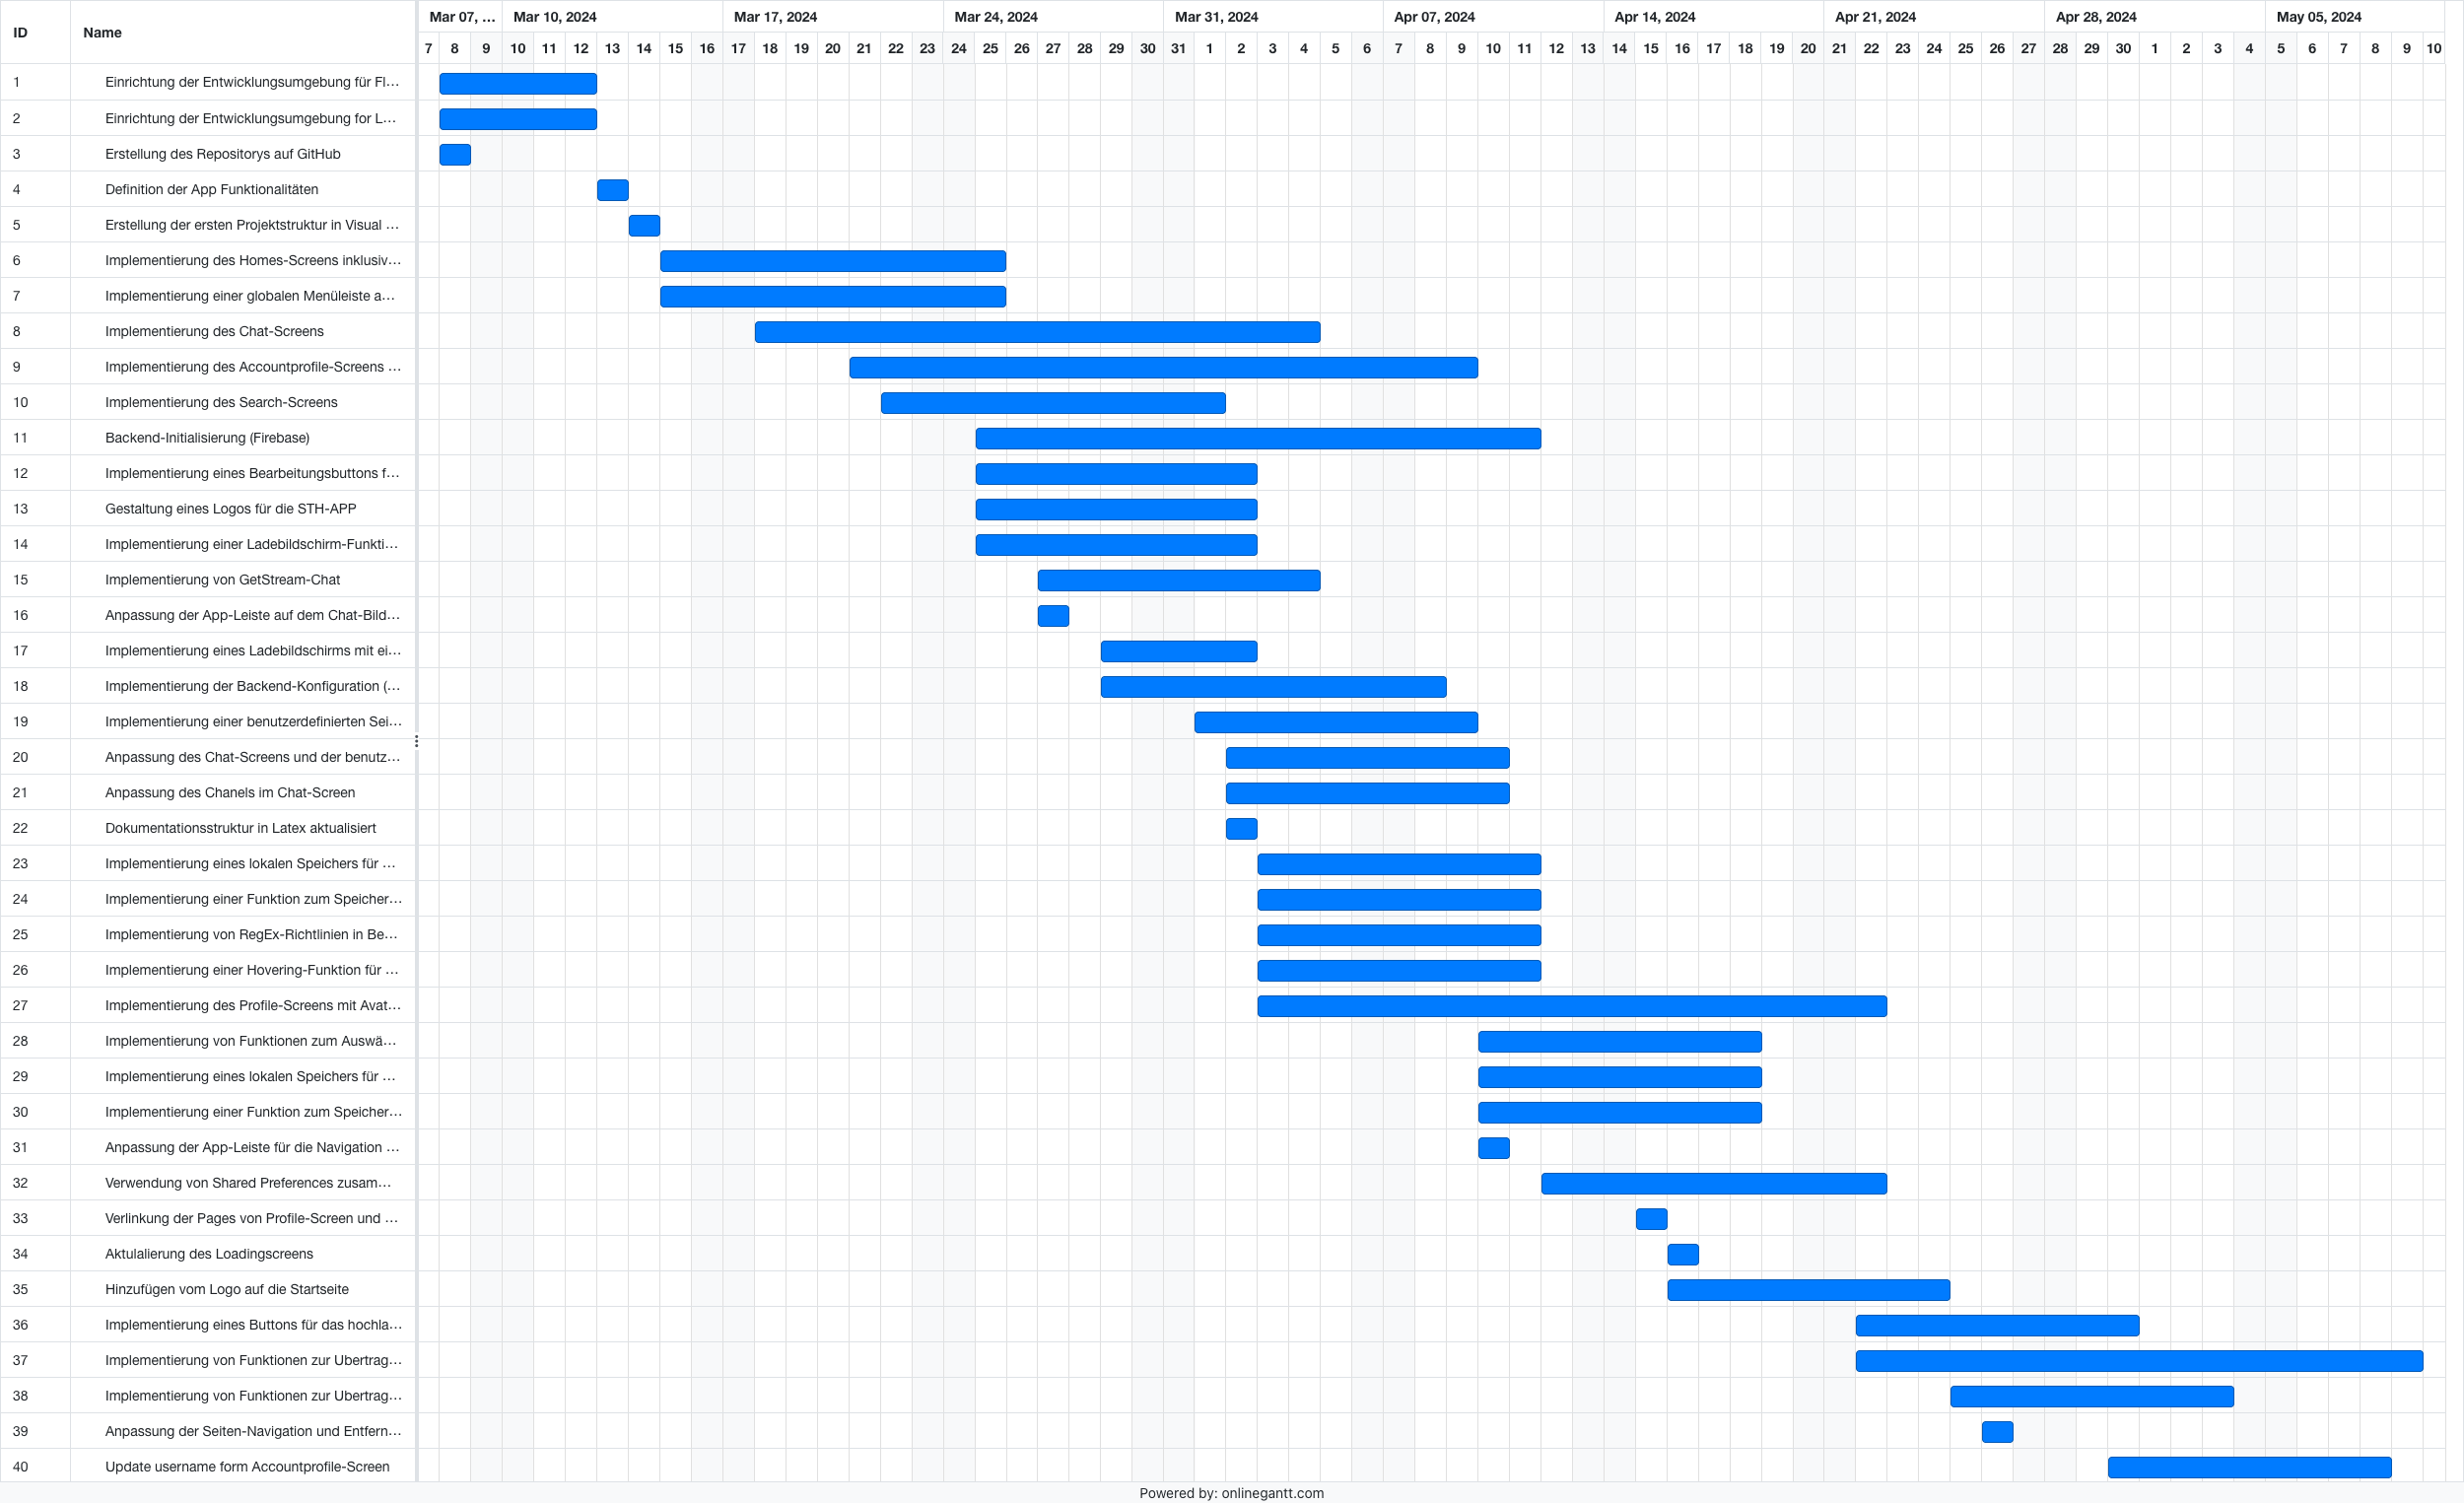
\includegraphics[width=0.9\textwidth]{assets/figures/STH GANTT Diagramm.png}
    \\
    Quelle: Eigene Darstellung über \url{https://www.onlinegantt.com}
\end{figure}
